\documentclass{article}
\usepackage[utf8x]{inputenc}
\usepackage{ucs}
\usepackage{amsmath} 
\usepackage{amsfonts}
\usepackage{marvosym}
\usepackage{wasysym}
\usepackage{upgreek}
\usepackage[english,russian]{babel}
\usepackage{graphicx}
\usepackage{float}
\usepackage{textcomp}
\usepackage{hyperref}
\usepackage{geometry}
  \geometry{left=2cm}
  \geometry{right=1.5cm}
  \geometry{top=1cm}
  \geometry{bottom=1.8cm}
\usepackage{tikz}
\usepackage{ccaption}
\usepackage{multicol}
\hypersetup{
   colorlinks=true,
   citecolor=blue,
   linkcolor=black,
   urlcolor=blue
}
\usepackage{listings}
\usepackage[absolute]{textpos}
\usepackage{colortbl,graphicx,tikz}
\definecolor{X}{rgb}{.5,.5,.5}


\begin{document}
\pagenumbering{gobble}
\lstdefinestyle{myCustomCStyle}{
  language=C,
  basicstyle=\linespread{1.1}\ttfamily,
  columns=fixed,
  fontadjust=true,
  basewidth=0.5em,
  keywordstyle=\color{blue}\bfseries,
  commentstyle=\color{gray},
  stringstyle=\ttfamily\color{orange!50!black},
  showstringspaces=false,
  numbersep=5pt,
  numberstyle=\tiny\color{black},
  numberfirstline=true,
  stepnumber=1,   
  numbersep=10pt,
  backgroundcolor=\color{white},
  showstringspaces=false,
  captionpos=b,
  breaklines=true,
  breakatwhitespace=true,
  xleftmargin=.2in,
  extendedchars=\true,
  keepspaces = true,
  upquote = true,
  emph = {size_t, NULL},
  emphstyle={\color{blue}\bfseries},
}


\lstdefinestyle{longCodeStyle}{
  style=myCustomCStyle,
  framexleftmargin=5mm, 
  frame=shadowbox, 
  rulesepcolor=\color{gray}
}

\lstset{style=myCustomCStyle}
\lstset{literate=%
   *{0}{{{\color{red!20!violet}0}}}1
    {1}{{{\color{red!20!violet}1}}}1
    {2}{{{\color{red!20!violet}2}}}1
    {3}{{{\color{red!20!violet}3}}}1
    {4}{{{\color{red!20!violet}4}}}1
    {5}{{{\color{red!20!violet}5}}}1
    {6}{{{\color{red!20!violet}6}}}1
    {7}{{{\color{red!20!violet}7}}}1
    {8}{{{\color{red!20!violet}8}}}1
    {9}{{{\color{red!20!violet}9}}}1
}
\newpage
\newgeometry{left=2cm,right=2cm,top=1cm,bottom=1.5cm}

\title{Семинар \#6: Динамический массив.\vspace{-5ex}}\date{}\maketitle

\section*{Разные варианты массивов в языке C}
\subsection*{Статический массив}
\begin{raggedleft}
\textit{Статический массив} -- это массив, размер которого фиксирован. В языке C такой массив создается так:
\end{raggedleft}
\begin{lstlisting}
int a[3] = {10, 20, 30};  
\end{lstlisting}
У такого статического массива есть 2 проблемы:
\begin{itemize}
\item Нельзя поменять размер, то есть нельзя добавить или удалить элемент.
\item Он выделяется на стеке и его максимальный размер сильно ограничен.
\end{itemize}


\subsection*{Массив на стеке с переменным размером, но фиксированной вместимостью}
Первую проблему можно частично решить, если создать массив больше, чем нужно на данный момент:
\begin{lstlisting}
int a[100] = {10, 20, 30};
size_t size = 3;
\end{lstlisting}
В этом примере мы создали статический массив, который может хранить 100 элементов, но в данный момент используем только первые 3 элемента. Чтобы помнить, сколько элементов используется в данный момент мы завели переменную \texttt{size}. Введём следующие определения:
\begin{itemize}
\item \textit{Размер массива (англ. size)} -- количество элементов массива, которые доступны для использования.
\item \textit{Вместимость массива (англ. capacity)} -- количество элементов, под которые в массиве выделена память.
\end{itemize}
То есть, для массива из примера выше размер равен 3, а вместимость равна 100.
В такой массив мы можем добавлять элементы, но только до тех пор пока размер меньше, чем вместимость. Например, добавить новый элемент в конец массива \texttt{a} можно так (но только если \texttt{size < 100}):
\begin{lstlisting}
a[size] = 60;
size += 1;
\end{lstlisting}
Несмотря на то, что в такой массив можно добавлять и удалять элементы, у такого подхода также есть недостатки. Вместимость не может меняться во время выполнения программы. Её нужно указать заранее. Если указать слишком маленькую вместимость, то этого может не хватить, а если указать слишком большую, то будет напрасно потрачено слишком много памяти. К тому же этот массив всё так же создаётся на стеке, поэтому его размер ограничен.

\subsection*{Выделение динамического массива в куче}
\textit{Динамический массив} -- это массив, размер и вместимость которого может меняться во время выполнения программы. Такой массив, можно создать, выделив память в куче:
\begin{lstlisting}
int* p = (int*)malloc(sizeof(int) * 3);
\end{lstlisting}
Указатель \texttt{p} указывает на массив из пяти элементов, созданный в куче.
После того, как такой массив был создан, можно изменить его размер. Для этого нужно сделать следующее:
\begin{enumerate}
\item Выделить в куче ещё один участок памяти под новый массив большего размера.
\item Скопировать данные из старого массива в новый.
\item Освободить память старого массива.
\end{enumerate}




\subsubsection*{Процесс увеличения размера массива, созданного в куче}


\noindent\begin{minipage}{.45\textwidth}
\begin{lstlisting}
1) Исходное положение

int* p = (int*)malloc(sizeof(int)*3);
p[0] = 10;
p[1] = 20;
p[3] = 30;
\end{lstlisting}
\end{minipage}
\begin{minipage}{.45\textwidth}
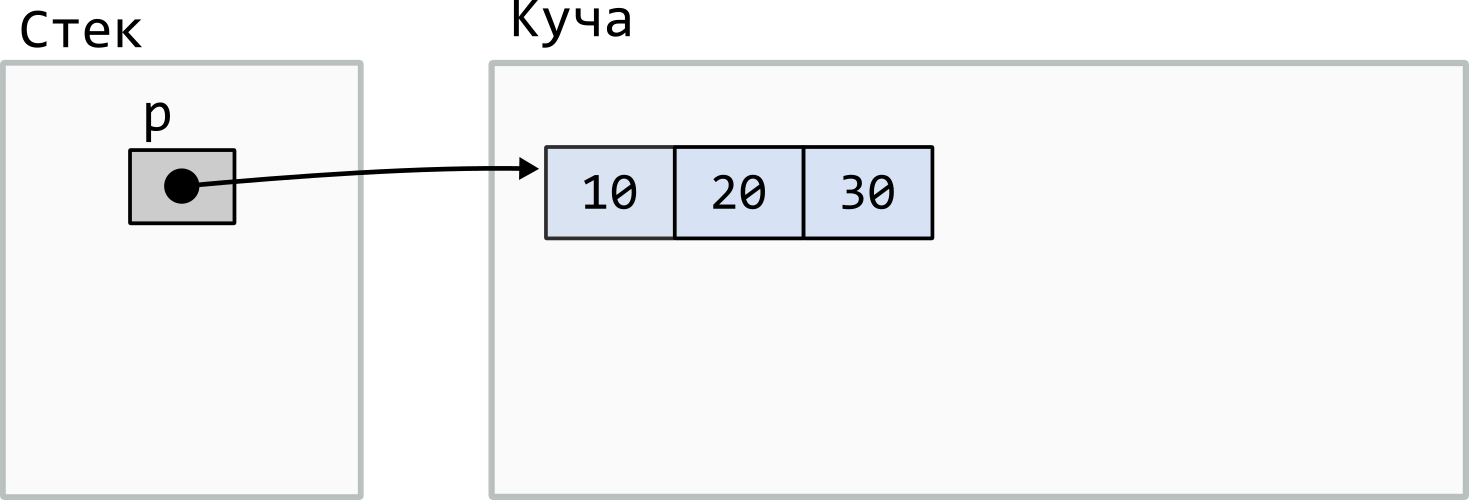
\includegraphics[scale=0.75]{../images/malloc_realocation1.png}
\end{minipage}
\quad\\
\quad\\
\quad\\


\noindent\begin{minipage}{.45\textwidth}
\begin{lstlisting}
2) Выделяем новый массив большей памяти

int* q = (int*)malloc(sizeof(int)*4);
\end{lstlisting}
\end{minipage}
\begin{minipage}{.45\textwidth}
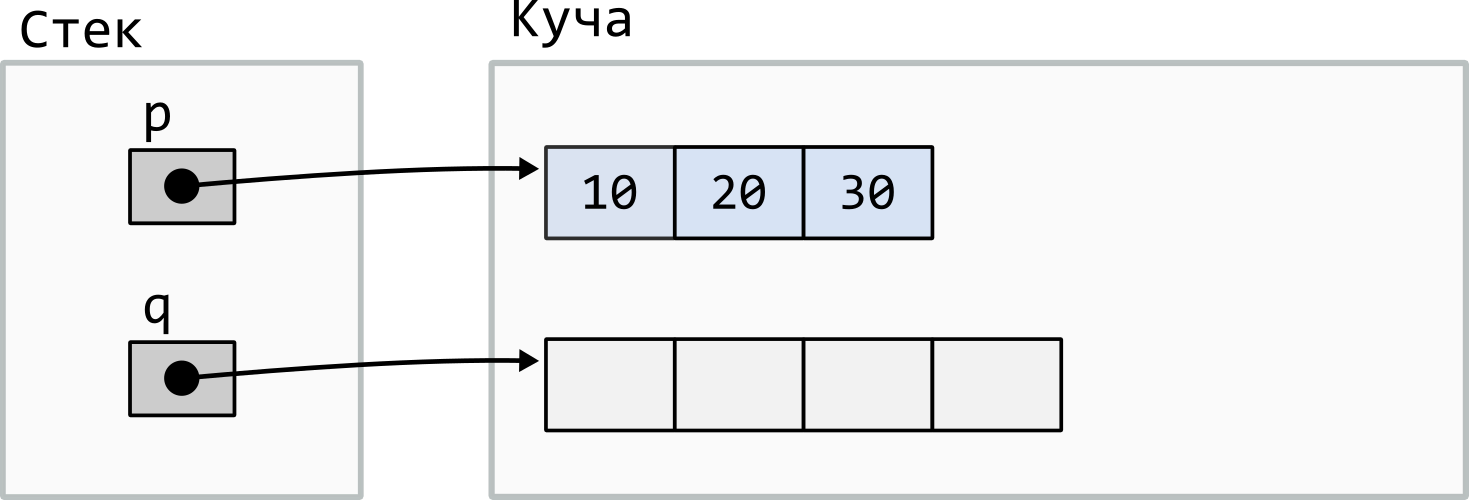
\includegraphics[scale=0.75]{../images/malloc_realocation2.png}
\end{minipage}
\quad\\
\quad\\
\quad\\


\noindent\begin{minipage}{.45\textwidth}
\begin{lstlisting}
3) Копируем элементы из старого массива
   и добавляем новый элемент
   
for (size_t i = 0; i < 3; ++i)
    q[i] = p[i];
q[3] = 40;
\end{lstlisting}
\end{minipage}
\begin{minipage}{.45\textwidth}
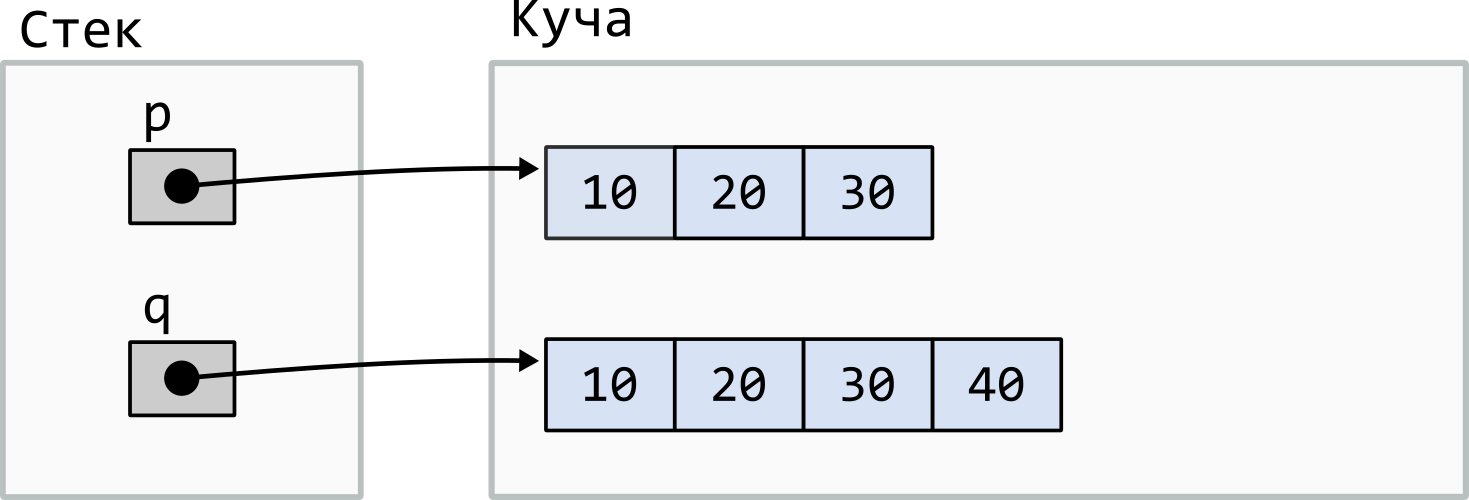
\includegraphics[scale=0.75]{../images/malloc_realocation3.png}
\end{minipage}
\quad\\
\quad\\
\quad\\


\noindent\begin{minipage}{.45\textwidth}
\begin{lstlisting}
4) Освобождаем память старого массива

free(p);
\end{lstlisting}
\end{minipage}
\begin{minipage}{.45\textwidth}
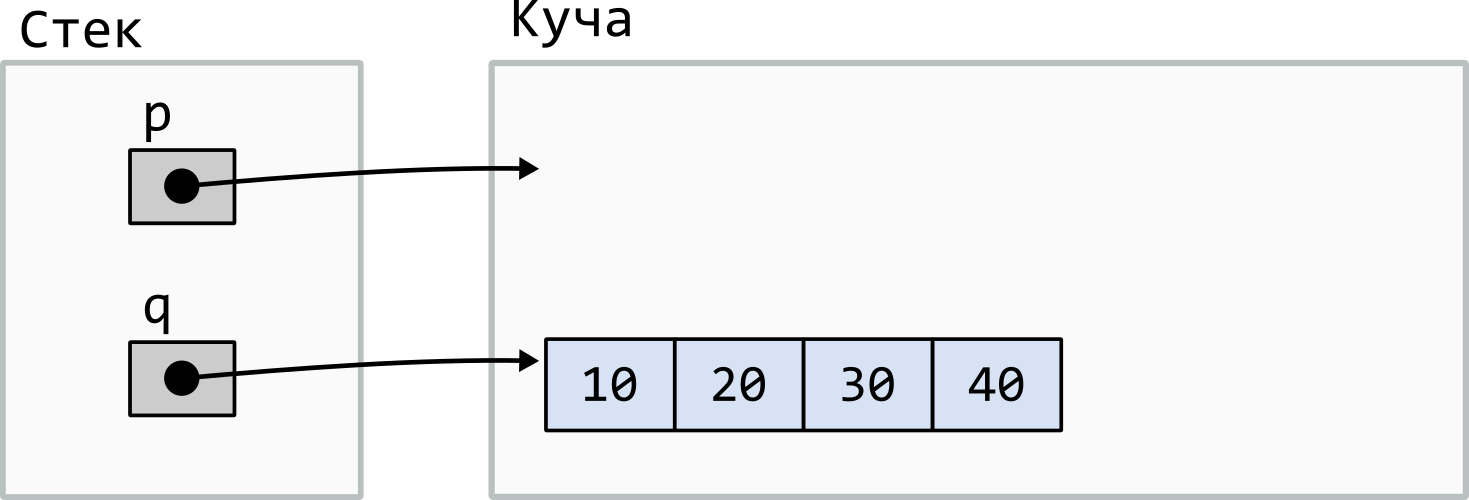
\includegraphics[scale=0.75]{../images/malloc_realocation4.png}
\end{minipage}
\quad\\
\quad\\
\quad\\


\noindent\begin{minipage}{.45\textwidth}
\begin{lstlisting}
5) Изменяем значение старого указателя

p = q;
\end{lstlisting}
\end{minipage}
\begin{minipage}{.45\textwidth}
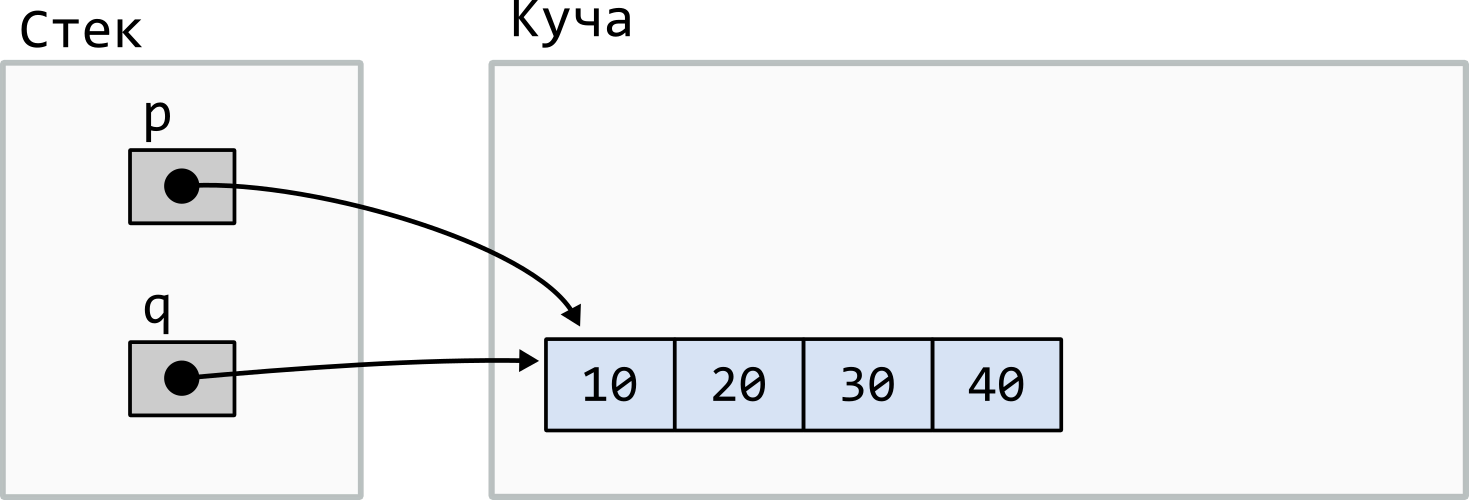
\includegraphics[scale=0.75]{../images/malloc_realocation5.png}
\end{minipage}
\quad\\
\quad\\
\quad\\

Такой подход позволяет создавать массивы с изменяемым размером, не ограниченным размером стека.
Однако, и этого подхода есть недостатки:
\begin{itemize}
\item Медленное добавление элементов. Для того, чтобы добавить один элемент в массив, нам пришлось вызвать \texttt{malloc}, так же скопировать весь массив.
\item Придётся делать все операции по выделению/освобождению памяти и копированию массива каждый раз, когда нужно изменить размер. Это неудобно.
\end{itemize}
Эти проблемы мы решим при написании своего динамического массива.

\newpage
\section*{Создаём свой динамический массив}

В отличии от многих других языков, в языке C нет удобного динамического массива, поэтому нам придётся написать свой. Попробуем написать наш массив так, чтобы он удовлетворял следующим требованиям:

\begin{enumerate}
\item В массив должно быть возможным добавление и удаление элементов. Его размер может меняться во время выполнения программы.
\item Размер массива не должен быть ограничен размером стека.
\item Массив должен быстро работать. Добавление и удаление элементов в конец массива должно работать за $O(1)$ в среднем. 
\item Массив не должен занимать слишком много памяти. А именно, общее количество выделенной для массива памяти должно быть не более чем в 2 раза превышать суммарный размер всех элементов массива.
\item С нашим массивом должно быть удобно работать.
\item Тип хранимого элемента массива должен быть настраиваемым.
\end{enumerate}
Структура для динамического массива будет выглядить следующим образом:
\begin{lstlisting}
struct dynarray 
{
    int* data;
    size_t size;
    size_t capacity;
};
typedef struct dynarray Dynarray;
\end{lstlisting}
Поля этой структуры:
\begin{itemize}
\item \texttt{data} -- указатель на элементы массива, которые выделяются в куче.
\item \texttt{size} -- текущий размер массива. Столько элементов содержится в массиве.
\item \texttt{capacity} - текущая вместимость массива. Под столько элементов в массиве выделена память. В отличии от статического массива эта величина может меняться. Количество памяти, выделенной в куче, будет равна \texttt{capacity * sizeof(int)}.
\end{itemize}
В памяти динамический массив с размером 5 и вместимостью 8 будет выглядеть следующим образом:
\begin{center}
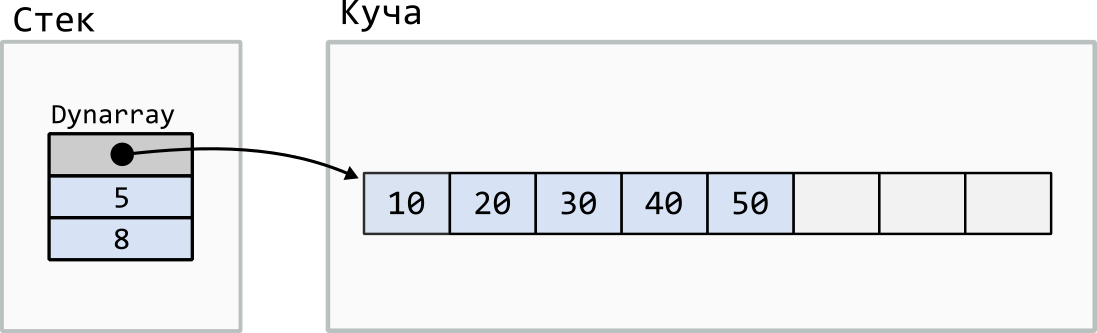
\includegraphics[scale=0.8]{../images/dynarray.png}
\end{center}

Напишем следующие функции для работы с нашим массивом:
\begin{lstlisting}
void init(Dynarray* pd, size_t n)               // Задаёт массив из n нулевых элементов
int  get(const Dynarray* pd, size_t i)          // Получает значение i - го элемента
void set(Dynarray* pd, size_t i, int value)     // Задаёт значение i - го элемента
void reserve(Dynarray* pd, size_t new_capacity) // Увеличивает вместимость массива
void push_back(Dynarray* pd, int value);        // Вставляет элемент в конец массива
void print(const Dynarray* pd)                  // Печатает массив на экран
void destroy(Dynarray* pd)                      // Уничтожает наш массив
\end{lstlisting}




\newpage
\subsection*{Процесс увеличения размера динамического массива}
\noindent\begin{minipage}{.40\textwidth}
\begin{lstlisting}
1) Исходное положение

Dynarray a;
init(&a, 3);
set(&a, 0, 10);
set(&a, 0, 20);
set(&a, 0, 30);
\end{lstlisting}
\end{minipage}
\begin{minipage}{.50\textwidth}
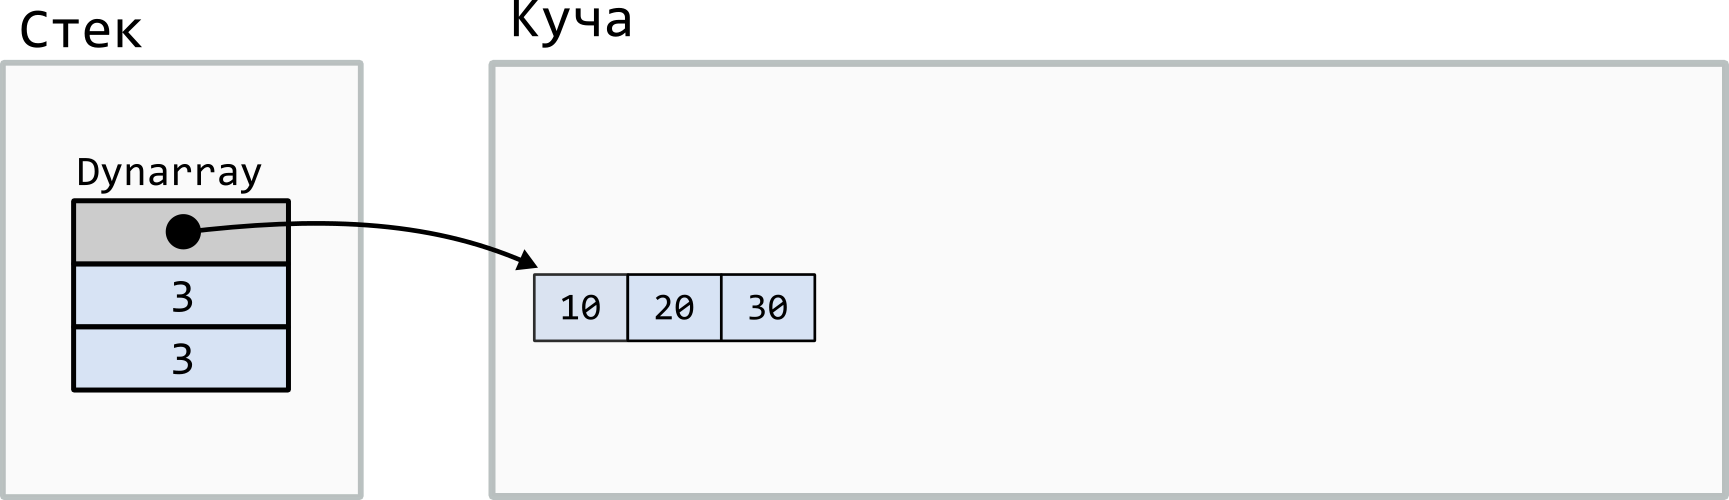
\includegraphics[scale=0.8]{../images/dynarray1.png}
\end{minipage}
\quad\\
\quad\\
\quad\\
\quad\\
\quad\\



\noindent\begin{minipage}{.40\textwidth}
\begin{lstlisting}
2) Добавляем один элемент, увеличивая размер массива, созданного в куче

push_back(&a, 40);
\end{lstlisting}
\end{minipage}
\begin{minipage}{.50\textwidth}
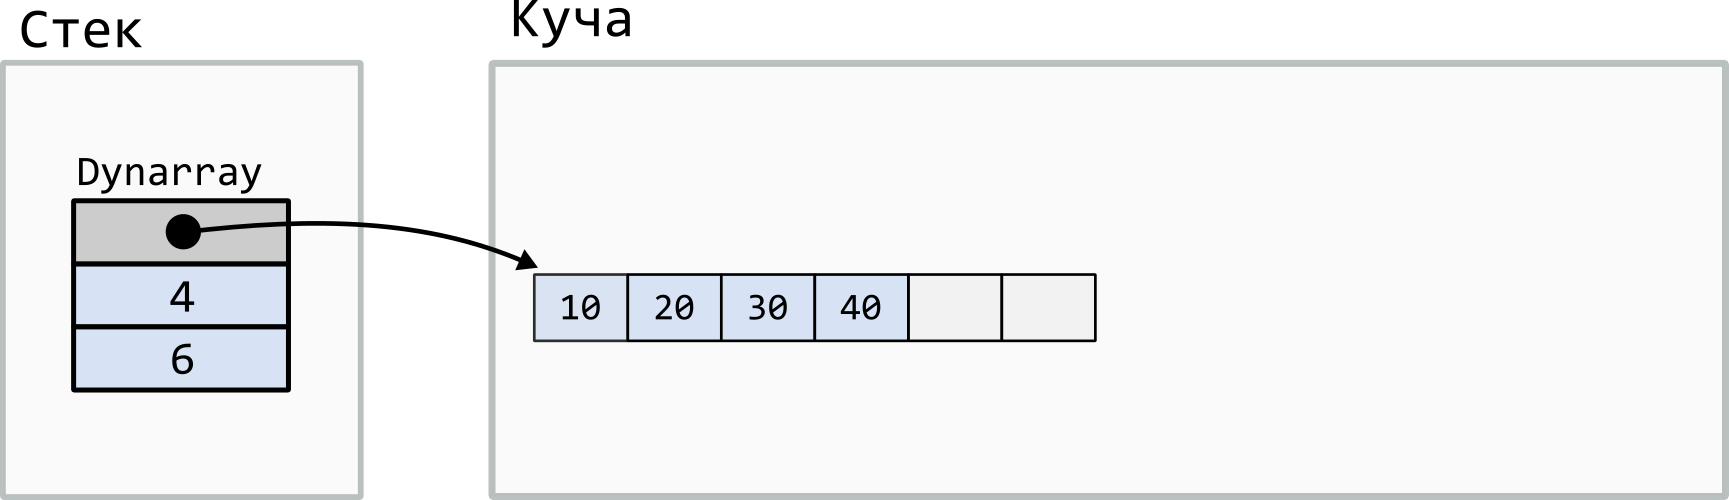
\includegraphics[scale=0.8]{../images/dynarray2.png}
\end{minipage}
\quad\\
\quad\\
\quad\\
\quad\\
\quad\\



\noindent\begin{minipage}{.40\textwidth}
\begin{lstlisting}
3) Добавляем ещё два элемента, на этот раз перевыделять память не нужно

push_back(&a, 50);
push_back(&a, 60);
\end{lstlisting}
\end{minipage}
\begin{minipage}{.50\textwidth}
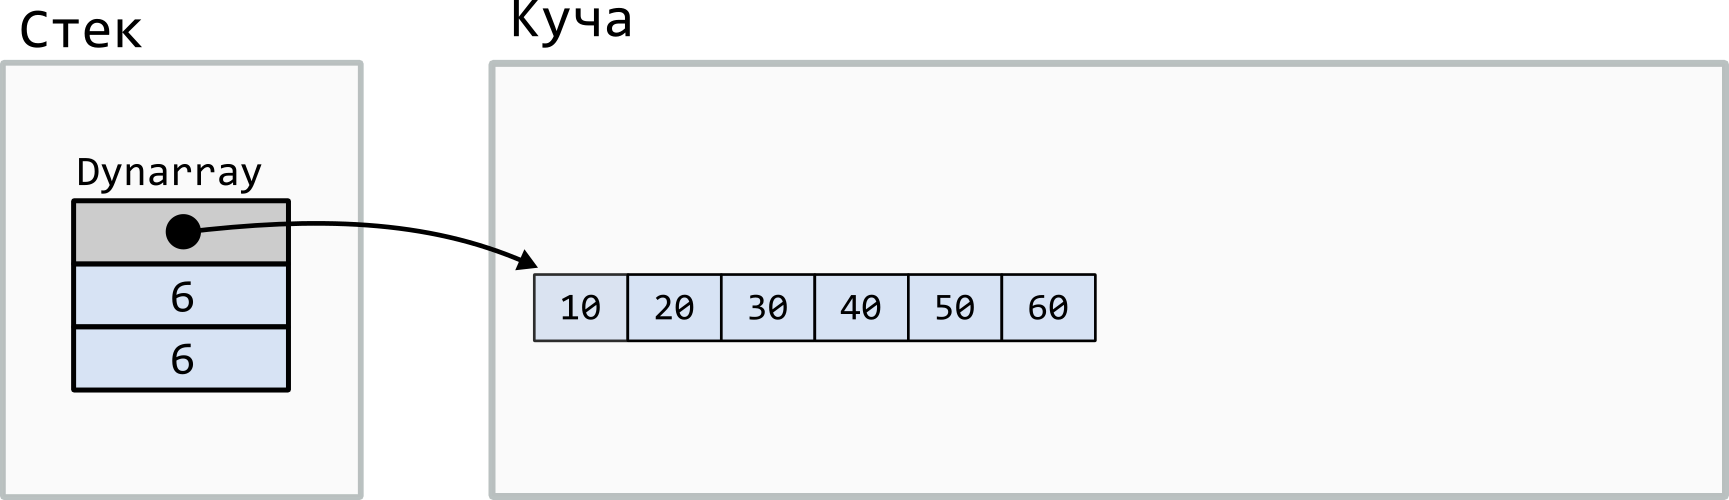
\includegraphics[scale=0.8]{../images/dynarray3.png}
\end{minipage}
\quad\\
\quad\\
\quad\\
\quad\\
\quad\\



\noindent\begin{minipage}{.40\textwidth}
\begin{lstlisting}
4) Добавляем ещё один элемент, увеличивая размер массива, созданного в куче

push_back(&a, 70);
\end{lstlisting}
\end{minipage}
\begin{minipage}{.50\textwidth}
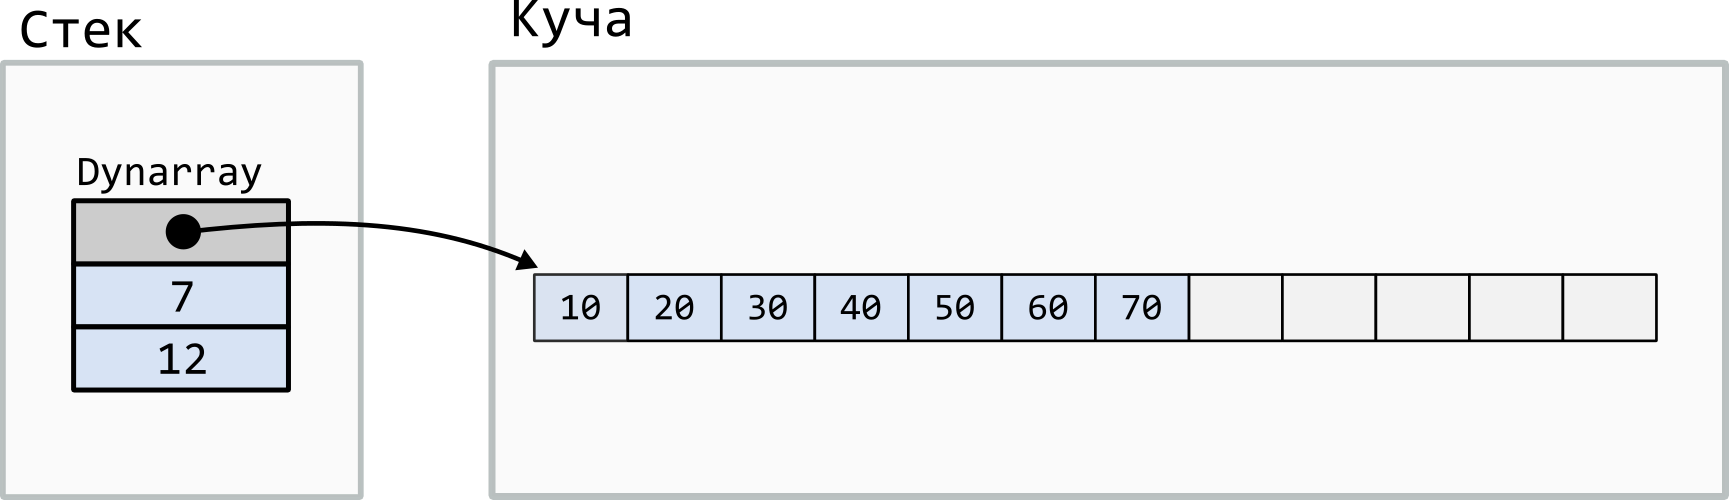
\includegraphics[scale=0.8]{../images/dynarray4.png}
\end{minipage}
\quad\\
\quad\\
\quad\\


\newpage
\subsection*{Исходный код нашего динамического массива}
Код также находится в файле \texttt{code/dynarray.c}.
\begin{lstlisting}[style=longCodeStyle]
#include <stdio.h>
#include <stdlib.h>
#include <assert.h>

// Error checked malloc
void* ecmalloc(size_t n)
{
    void* p = malloc(n);
    if (p == NULL)
    {
        fprintf(stderr, "Memory allocation error.\n");
        exit(1);
    }
    return p;
}

struct dynarray 
{
    int* data;
    size_t size;
    size_t capacity;
};
typedef struct dynarray Dynarray;

void clear(Dynarray* pd)
{
    for (size_t i = 0; i < pd->size; ++i)
        pd->data[i] = 0;
}

void init(Dynarray* pd, size_t initial_size) 
{
    pd->size = initial_size;
    pd->capacity = initial_size;
    if (pd->size == 0)
        pd->data = NULL;
    else
        pd->data = (int*)ecmalloc(pd->capacity * sizeof(int));
    clear(pd);
}

int get(const Dynarray* pd, size_t index) 
{
    assert(index >= 0 && index < pd->size);
    return pd->data[index];
}

void set(Dynarray* pd, size_t index, int value) 
{
    assert(index >= 0 && index < pd->size);
    pd->data[index] = value;
}

void reserve(Dynarray* pd, size_t new_capacity)
{
    if (new_capacity <= pd->capacity)
        return;

    int* new_data = (int*)ecmalloc(new_capacity * sizeof(int));
    for (size_t i = 0; i < pd->size; ++i)
        new_data[i] = pd->data[i];
        
    free(pd->data);
    pd->data = new_data;
    pd->capacity = new_capacity;
}

void push_back(Dynarray* pd, int x) 
{
    static const double growth_factor = 2;
    if (pd->size == pd->capacity) 
    {
        size_t new_capacity = (size_t)(growth_factor * pd->capacity);
        if (new_capacity <= pd->size)
            new_capacity = pd->size + 1;

        reserve(pd, new_capacity);
    }
    pd->data[pd->size] = x;
    pd->size += 1;
}

void print(const Dynarray* pd) 
{
    printf("dynarray: ");
    for (size_t i = 0; i < pd->size; ++i) 
        printf("%i ", pd->data[i]);
    printf("\n");
}

void destroy(Dynarray* pd) 
{
    free(pd->data);
    pd->data = NULL;
}

int main() 
{
    Dynarray a;
    init(&a, 0);
    for (int i = 0; i < 100; ++i)
        push_back(&a, i);
    print(&a);
    destroy(&a);
}
\end{lstlisting}



\newpage
\subsection*{Пояснение по исходному коду динамического массива}

\begin{itemize}
\item Была написана функция \texttt{ecmalloc}. Это просто \texttt{malloc} с проверкой на ошибки. В случае если \texttt{malloc} вернёт \texttt{NULL}, эта функция напечатает сообщение об ошибке и выйдет из программы. Функция печатает в стандартный поток \texttt{stderr}, предназначенный для вывода сообщений об ошибках.

\item Динамический массив передаётся в функции по указателю или по константному указателю в зависимости от того будет ли меняться массив в функции или нет. При этом, тут мы передаём по неконстантному указателю даже если поля структуры \texttt{Dynarray} не меняется, но меняются элементы в куче. Например, в функцию \texttt{set} динамический массив передаётся не по константному указателю, а по обычному.

\item Макрос \texttt{assert} или библиотеки \texttt{assert.h} -- это простой, но эффективный способ для обнаружения ошибок. Assert с английского переводится как "утверждать". Макрос \texttt{assert} принимает на вход условие. Если условие истинно, то \texttt{assert} ничего не делает, но если условие ложно, то \texttt{assert} печатает сообщение об ошибке и выходит из программы. Например, следующая строка:
\begin{lstlisting}
assert(index >= 0 && index < pd->size);
\end{lstlisting}
завершит программу с ошибкой, если \texttt{index} не принадлежит отрезку \texttt{[0, pd->size - 1]}.


\item Функция \texttt{init} создаёт массив из нулевых элементов размера \texttt{initial\_size}. Отдельно обрабатывается случай массива размера \texttt{0}. В этом случае память в куче не будет выделяться, а поле \texttt{data} будет равно \texttt{NULL}.

\item Функция \texttt{reserve} увеличивает вместимость массива до значения \texttt{new\_capacity}. Если вместимость уже больше или равна \texttt{new\_capacity}, то это функция ничеко не делает.

\item Функция \texttt{push\_back} добавляет один элемент в конец массива. Если вместимости массива не хватает, то эта функция вызывает \texttt{reserve}, чтобы увеличить вместимость в 2 раза (за исключением случая, когда вместимость равна 0, в этом случае новая вместимость будет равна 1). 
\end{itemize}



\subsection*{Стратегии роста вместимости динамического массива}
Если в нашем массиве перестёт хватать места, то его вместимость увеличивается в 2 раза. В принципе, можно было выбрать и другую стратегию выделения памяти.

\begin{itemize}
\item \textbf{Аддитивная стратегия} -- при нехватки места вместимость увеличивается на фиксированное количество элементов, например, на 100 элементов.
\item \textbf{Мультипликативная стратегия} -- при нехватки места вместимость увеличивается в фиксированное число раз, например, в 2 раза. Коэффициент увеличения вместимости массива называют фактором роста (англ. \textit{growth factor}). Обычно фактор роста выбирают равным 1.5 или 2.
\end{itemize}
Посчитаем среднюю вычислительную сложность добавления элемента в конец массива при использовании той или иной стратегии. Предположим, что изначально массив пуст, а затем мы добавляем в него $N$ элементов по одному, где $N$ очень большое. При каждом перевыделении памяти нам нужно скопировать элементы из старого массива в новый. 

В случае аддитивной стратегии с увеличением на 100 нам придется сделать:
$$
100 + 200 + 300 + ... + N = \frac{N^2}{200} 
$$
копирований элементов. В среднем, на одно добавление элемента придётся $\frac{N}{200}$ копирований. То есть, средняя вычислительная сложность в данном случае будет равна $O(N)$.

В случае мультипликативной стратегии с фактором роста 2 нам придется сделать:
$$
1 + 2 + 4 + 8 + ... + N = 2 \cdot N - 1
$$
копирований элементов. В среднем, на одно добавление элемента придётся $2$ копирования. То есть, средняя вычислительная сложность в данном случае будет равна $O(1)$.

Мультипликативная стратегия лучше в общем случае. Аддитивную стратегию можно использовать, если известно, что массив не будет часто расширяться и его размер всегда будет находится в некотором заранее известном интервале. В этом случае, использование аддитивной стратегии будет более эффективно по памяти.


\newpage
\section*{Директивы препроцессора}

\subsection*{Директива \texttt{\#include}}

\subsection*{Заголовочные файлы}

\subsection*{Проблема двойного включения}
Стражи включения и директива \texttt{\#pragma once}.

\subsection*{Директивы макросов \texttt{\#define}}

\subsection*{Директивы условной компиляции}
\texttt{\#if}, \texttt{\#else}, \texttt{\#elif}, 
\texttt{\#ifdef}, \texttt{\#ifndef}, \texttt{\#endif}.


\subsection*{Флаг \texttt{-D} для компилятора \texttt{gcc}}

\subsection*{Стандартные макро-константы}
\begin{verbatim}
__FILE__
__LINE__
__DATE__
__TIME__
__cplusplus
_WIN32
_WIN64
_MSC_VER
__MINGW32__
\end{verbatim}

\begin{lstlisting}
#include <stdio.h>

int main()
{
#ifdef _WIN32
    printf("Windows\n");
#elif __linux__
    printf("Linux\n");
#elif __APPLE__
    printf("Apple\n");
#endif
}
\end{lstlisting}


\newpage
\section*{Функциональные макросы}

Многострочные макросы. Типичные ошибки, которые
могут возникнуть при работе с функциональными макросами. 
Макросы \texttt{SUM}, \texttt{MULT}. Передача \texttt{i++} в макрос \texttt{SQUARE}.
Макросы, содержащие другие макросы.

Использование оператора \texttt{do while} в
многострочных функциональных макросах. Операция стрингификация (\texttt{\#}). Операция конкатенация (\texttt{\#\#}).
Макрос \texttt{assert} из библиотеки \texttt{assert.h}. Написание макроса, аналогичного макросу \texttt{assert}. Флаг \texttt{-E} компилятора \texttt{gcc}.

\newpage
\section*{Односвязный список}

\textit{Односвязный список} -- базовая динамическая структура данных, состоящая из узлов, содержащих указатели на следующий узел списка. В отличии от массива элементы связного списка не лежат в памяти вплотную друг к другу. В качестве узла выступает структура, которая хранит элемент и указатель на следующий узел, например, вот такая:
\begin{lstlisting}
struct node 
{
    int value;
    struct node* next;
};
typedef struct node Node;
\end{lstlisting}

Для того, чтобы было удобно работать со связным списком также создадим структуру для самого списка. В простейшем случае она будет хранить указатель на первый узел:
\begin{lstlisting}
struct forwardlist 
{
    Node* head;
};
typedef struct forwardlist ForwardList;
\end{lstlisting}

В программе будем называть односвязный список как \texttt{ForwardList}, так как по нему можно перемещаться только вперёд. В памяти односвязный список будет выглядеть так:
\begin{center}
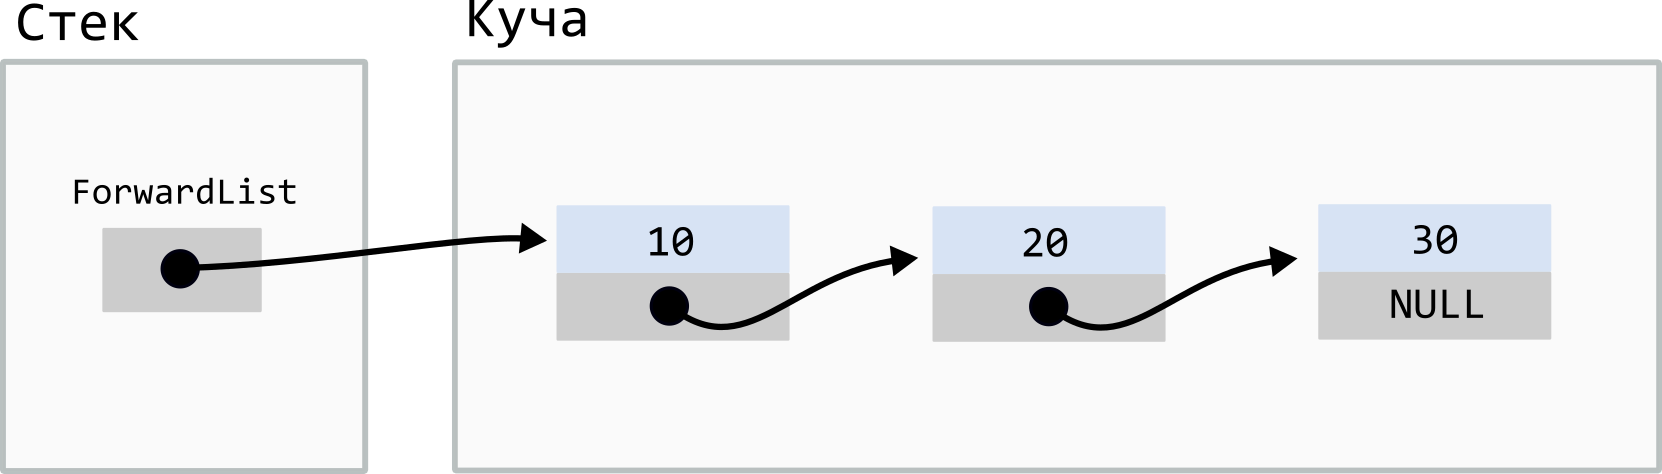
\includegraphics[scale=0.85]{../images/forward_list.png}
\end{center}





\iffalse
\newpage
\subsection*{Задачи:} 
Напишите следующие функции для работы с динамическим массивом:
\begin{itemize}
\item \texttt{Dynarray dynarray\_create(size\_t initial\_capacity)} -- эта функция должна создавать динамический массив с размером равным нулю и вместимостью равной \texttt{initial\_capacity}. Память должна выделяться в куче с помощью \texttt{malloc}.

\item \texttt{void dynarray\_destroy(Dynarray* d)} -- эта функция должна освобождать выделенную память (\texttt{free}).

\item Перепишите все функции из прошлой части: \texttt{dynarray\_push\_back}, \texttt{dynarray\_print} и другие.

\item \textbf{Расширение массива:} Измените код так, чтобы происходило перевыделение памяти тогда, когда размер массива начинает превышать вместимость в функциях \texttt{dynarray\_push\_back} и \texttt{dynarray\_insert}. Вместимость динамического массива должна увеличиваться в 2 раза.  Это можно сделать двумя способами:
\begin{itemize}
\item Выделить новый участок памяти в 2 раза больше прежнего, используя \texttt{malloc}. Переписать все элементы в новую память. Освободить старую память с помощью \texttt{free}.
\item Использовать функцию \texttt{realloc}, которая будет делать то же самое, но более эффективно.
\end{itemize}

\item \textbf{Проверка на корректность:} Функции \texttt{malloc} и \texttt{realloc} не всегда могут выделить необходимую память. Например, если вы запросите больше чем вся оперативная память, то они ничего не смогут сделать. В этом случае эти функции возвращают нулевой указатель (т.е. указатель, равный \texttt{NULL}). В случае возникновения такой ошибки \texttt{realloc} не освобождает старую память. Добавьте в программу проверки на возникновения таких ошибок. Если память выделить нельзя, то программа должна печатать сообщение о нехватке памяти и завершаться.

\item \textbf{Размер и вместимость:}
Напишите программу, которая будет создавать стек вместимости \texttt{1} и добавлять в него последовательно \texttt{200} элементов. При каждом добавлении элемента печатайте размер и вместимость.\\

\item \textbf{Другие типы элементов:} Предположим, что вы однажды захотите использовать динамический массив не для целочисленных чисел типа \texttt{int}, а для какого-нибудь другого типа (например \texttt{char}). Введите синоним для типа элементов динамического массива:
\begin{verbatim}
typedef int Data;
\end{verbatim}
Измените тип элемента динамического массива во всех функциях с \texttt{int} на \texttt{Data}. Теперь вы в любой момент сможете изменить тип элементов стека, изменив лишь одну строчку.
\end{itemize}


\newpage
\section*{Заголовочные файлы}


\newpage
\section*{Абстрактные типы данных: Стек и Очередь}
\textbf{Абстракстный тип данных (АТД)} - это математическая модель для типов данных, которая задаёт поведение этих типов, но не их внутреннею реализацию.\\

\textbf{Стек (Stack, не путайте с сегментом памяти под таким же названием!)} - это АТД, который представляет собой коллекцию элементов, менять которые можно только с помощью двух операций:
\begin{itemize}
\item \texttt{push} - добавить элемент в стек.
\item \texttt{pop} - извлечь из стека последний добавленный элемент.
\end{itemize}
Таким образом, поведение стека задаётся этими двумя операциями. Так как стек - это абстрактный тип данных, то его внутренняя реализация на языке программирования может быть самой разной. Стек можно сделать на основе статического массива, на основе динамического массива или на основе связного списка. Внутренняя реализация не важна, важно только наличие операций \texttt{push} и \texttt{pop}. \\
Не нужно путать абстракстный тип данных стек с сегментом памяти стек.\\

\textbf{Очередь (Queue)} - это АТД, который представляет собой коллекцию элементов, менять которые можно только с помощью двух операций:
\begin{itemize}
\item \texttt{enqueue} - добавить элемент в очередь.
\item \texttt{dequeue} - извлечь из очереди первый добавленный элемент из оставшихся.
\end{itemize}

\begin{center}
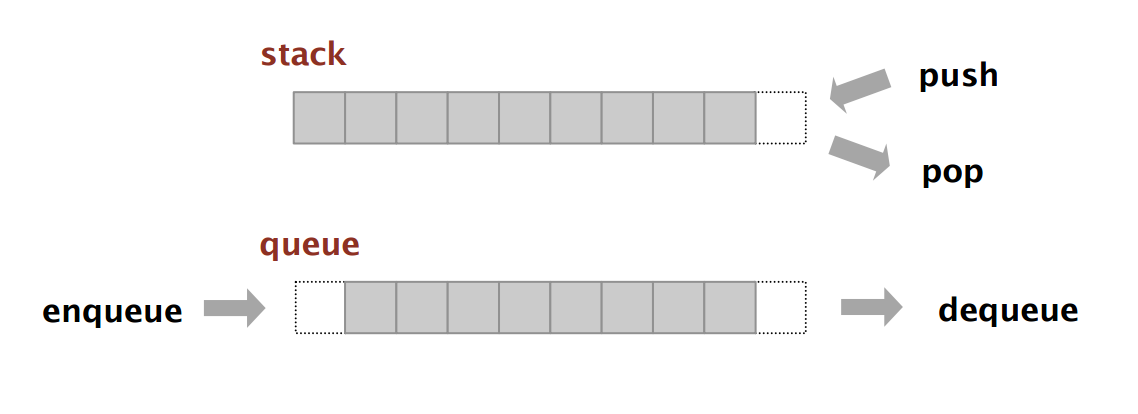
\includegraphics[scale=0.31]{../images/stack_queue.png}
\end{center}

\textbf{Дек (Deque = Double-ended queue)} - это АТД, который представляет собой коллекцию элементов, менять которые можно только с помощью четырёх операций:
\begin{itemize}
\item \texttt{push\_back} - добавить элемент в конец.
\item \texttt{push\_front} - добавить элемент в начало.
\item \texttt{pop\_back} - извлечь элемент с конца.
\item \texttt{pop\_front} - извлечь элемент с начала.\\
\end{itemize}

\textbf{Очередь с приоритетом (Priority Queue)} - это АТД, который представляет собой коллекцию элементов, менять которые можно только с помощью двух операций:
\begin{itemize}
\item \texttt{insert} - добавить элемент.
\item \texttt{extract\_best} - извлечь из очереди элемент с наибольшим приоритетом. 
\end{itemize}
То, что будет являться приоритетом может различаться. Это может быть как сам элемент, часть элемента (например, одно из полей структуры) или другие данные, подаваемые на вход операции \texttt{insert} вместе с элементом. В простейшем случае, приоритетом является сам элемент (тогда очередь с приоритетом просто возвращает максимальный элемент) или сам элемент со знаком минус (тогда очередь с приоритетом возвращает минимальный элемент).


\newpage
\section*{Реализация стека на основе динамического массива}

\begin{center}
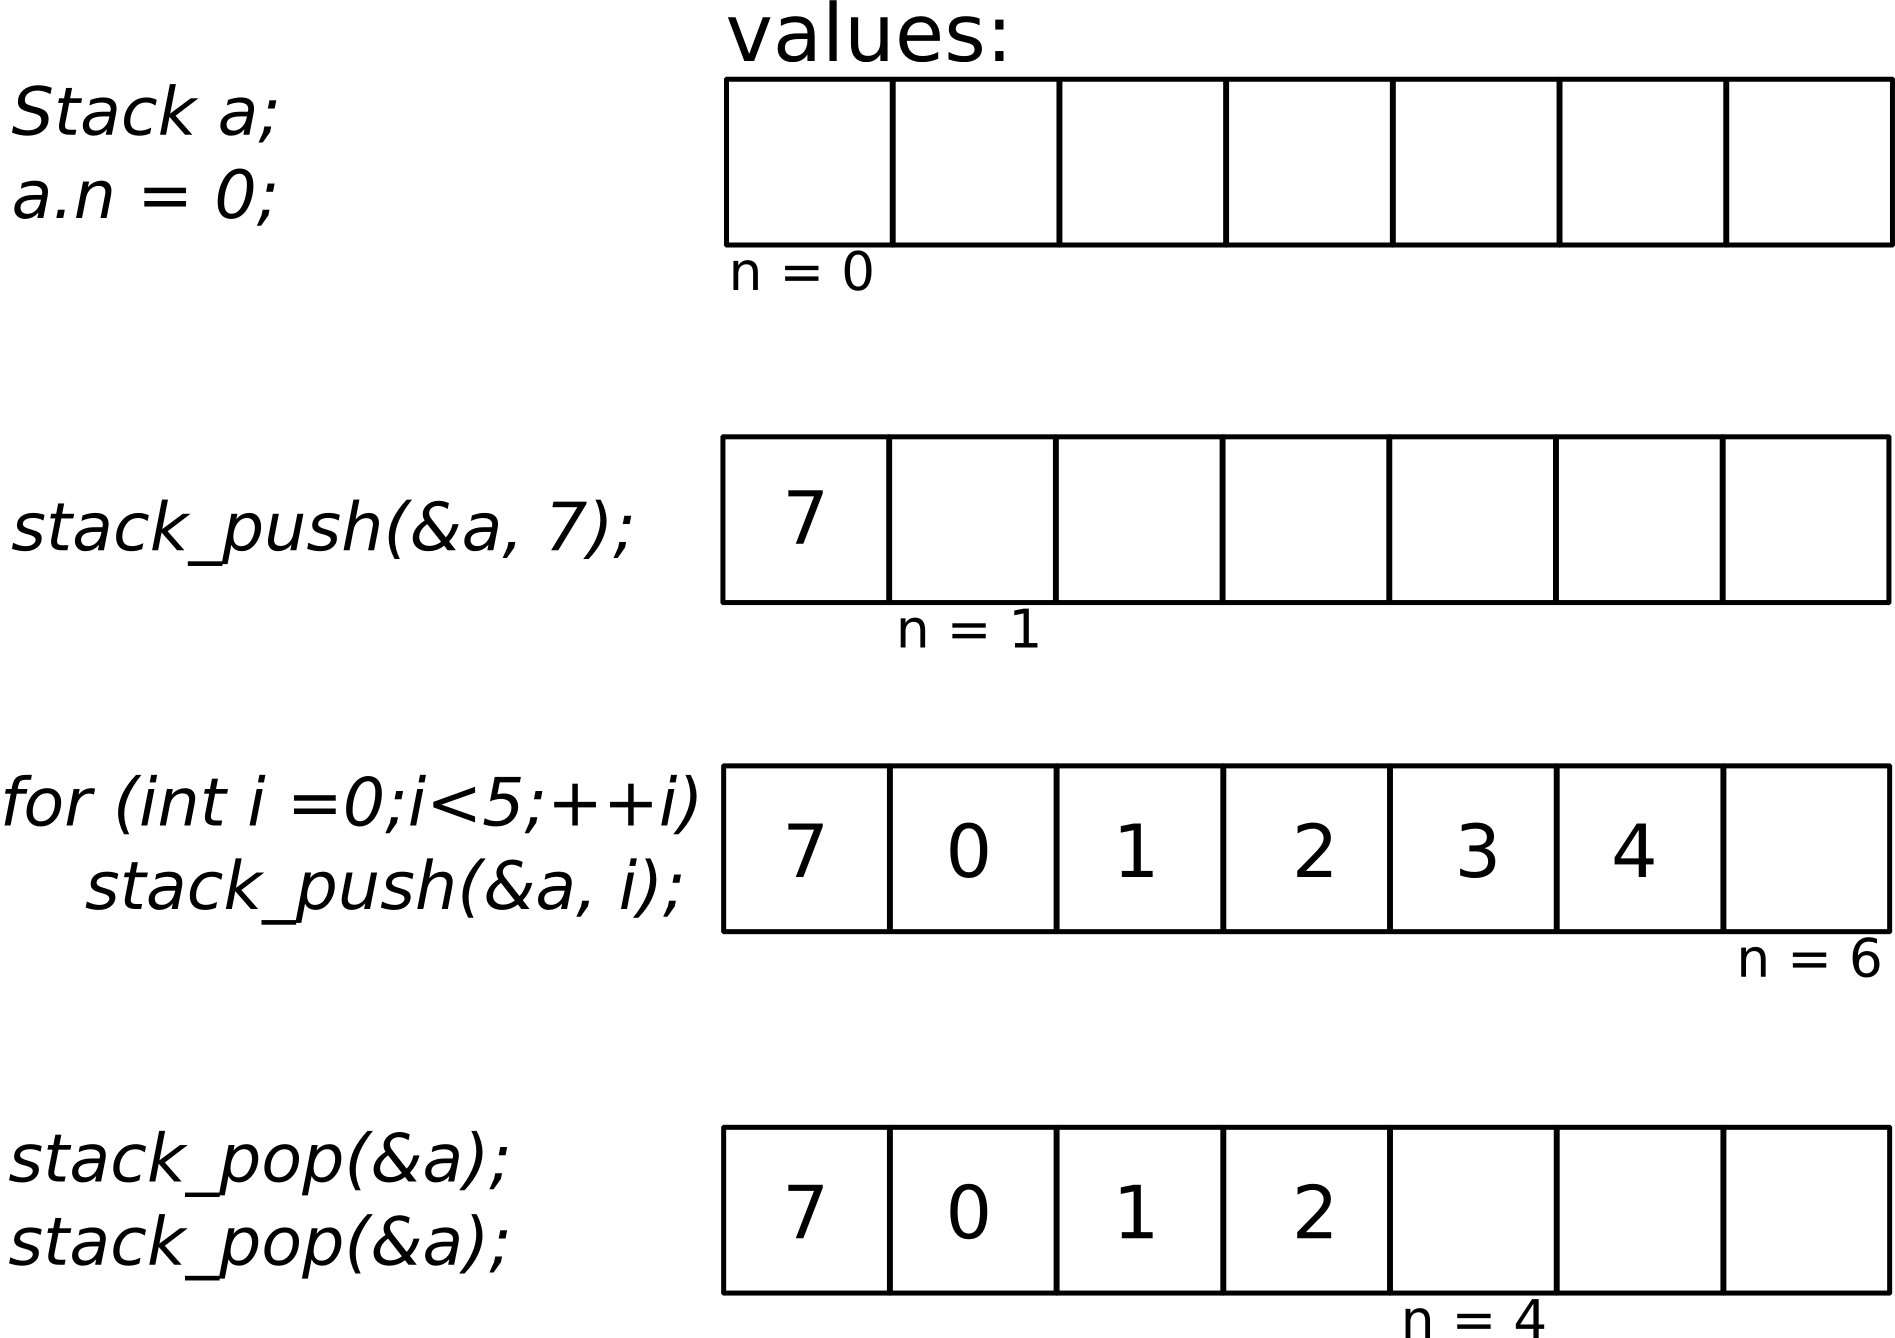
\includegraphics[width=0.6\linewidth]{../images/stack.png}
\end{center}

\subsection*{Задачи:}
\begin{itemize}
\item Напишите следующие функции:
\begin{enumerate}
\item \texttt{void stack\_push(Stack* s, Data x)} -- добавляет элемент в стек.
\item \texttt{Data stack\_get(const Stack* s)} -- возвращает элемент, находящийся в вершине стека, но не изменяет стек.
\item \texttt{void stack\_pop(Stack* s)} -- удаляет элемент, находящийся в вершине стека. 
\item \texttt{int stack\_is\_empty(const Stack* s)} -- возвращает 1 если стек пуст и 0 иначе.
\item \texttt{void stack\_print(const Stack* s)} -- распечатывает все элементы стека.
\end{enumerate}



\item \textbf{Скобочки}: Написать программу которая будет считывать последовательность скобочек и
печатать \texttt{Yes} или \texttt{No} в зависимости от того является ли эта последовательность допустимой. Для считывания строки: \texttt{scanf(``\%s'', str);}
\begin{multicols}{2}
\begin{center}
\begin{tabular}{ c | c }
 вход & выход \\ \hline
 \texttt{()} & Yes \\
 \texttt{\{[()]\}} & Yes  \\ 
 \texttt{)))))}  &  No \\ 
 \texttt{([)]}  &  No \\ 
 \texttt{[\{\}()]}  &  Yes \\ 
\end{tabular}
\end{center}

\begin{center}
\begin{tabular}{ c | c }
 вход & выход \\ \hline
 \texttt{)(}  &  No \\
 \texttt{((((((()))))))} & Yes \\
 \texttt{\{\{\{\{} & No  \\ 
 \texttt{\{[([]()[\{\}])][()]\}}  &  Yes \\ 
 \texttt{]}  &  No \\ 
\end{tabular}
\end{center}
\end{multicols}


\item \textbf{Следующий больший}: На вход поступает последовательность чисел. Нужно найти, для каждого элемента, индекс первого элемента, который следует после данного и является больше данного. Если такого элемента нет, то нужно напечатать \texttt{-1}.
\begin{center}
\begin{tabular}{ l | l }
 вход & выход \\ \hline
 \texttt{10} &  \texttt{1 4 3 4 5 -1 7 -1 -1 -1}\\
 \texttt{1 5 2 4 6 9 1 8 7 3} & \\ \hline
 
 \texttt{5} &  \texttt{1 2 3 4 -1}\\
 \texttt{1 2 3 4 5} & \\ \hline
 
  \texttt{2} &  \texttt{-1 -1}\\
 \texttt{2 1} & \\
\end{tabular}
\end{center}

\end{itemize}




\section*{Массив фиксированного размера внутри структуры}
В файле \texttt{0array\_in\_struct.c} содержится минимальный пример массива, который хранится внутри структуры. Максимальная вместимость массива равна \texttt{100}. А размер хранится внутри структуры и может принимать значения от 0 до 100. Функция \texttt{push\_back} принимает на вход адрес на такую структуру и число \texttt{value}, а затем добавляет это число в конец массива.\\

Зачем хранить массив внутри структуры, если можно было бы просто создать его без струтуры? На самом деле у такого подхода много преимуществ:
\begin{enumerate}
\item Он позволяет нам самим описать поведение массива при добавлении и удалении элементов.
\item Мы можем передавать такой массив внутри функций также как и обычные переменные.
\item Такой подход распространяется на более сложные структуры данных
\end{enumerate}

\subsection*{Задачи:} 
Напишите следующие функции для работы с этим массивом:
\begin{itemize}
\item \texttt{array\_print} -- эта функция должна принимать на вход адрес структуры \texttt{Array} и печатать массив на экран.
\item \texttt{array\_is\_empty} -- эта функция должна принимать на вход адрес структуры \texttt{Array} и возвращать \texttt{1}, если массив пуст и \texttt{0} иначе.
\item \texttt{int array\_get(const Array* a, int index)} эта функция должна возвращать число, которое лежит по индексу \texttt{index} в массиве.
\item \texttt{void array\_set(const Array* a, int index, int value)} -- эта функция должна устанавливать элемент массива, лежащий по индексу \texttt{index} значением \texttt{value}.
\item \texttt{void array\_erase(const Array* a, int index)} -- эта функция должна удалять элемент под индексом \texttt{index}. При этом, конечно, все элементы, которые следовали после удаляемого нужно сместить влево на 1 элемент.
\item \texttt{void array\_insert(const Array* a, int index)} -- эта функция должна вставлять элемент в массив в место между элементами с индексами \texttt{index - 1} и \texttt{index}. При этом, конечно, все элементы, которые находились правее этого места, должны сместиться вправо на один элемент.
\item \texttt{void array\_append(Array* a, const Array* b)} -- эта функция должна добавлять всё содердимое массива \texttt{b} в конец массива \texttt{a}.

\item \textbf{Проверка индекса:} Как известно, в языке \texttt{C} у статических массивов нет проверки на выход за пределы массива. Например, следующий код может сработать и не выдасть никакой ошибки.
\begin{lstlisting}
int array[100] = {};
printf("%i\n", array[101]);
\end{lstlisting}
Компилятор просто преобразует строку \texttt{array[101]} в \texttt{*(array + 101)} и обратится к соответствующему участку памяти.
Причина того, что в \texttt{C} нет такой проверки заключается в том, что она бы немного замедлила программу. Язык \texttt{C} ориентирован на максимальное быстродействие, поэтому и не делает такую проверку. 

Однако, за отсутствие такой проверки приходится платить тем что в программе могут появиться сложно выявляемые ошибки. Например, если вы случайно ошибётесь с индексами массива, то можете этого даже не заметить. Программа будет работать с памятью за пределами этого массива и почти всегда выдавать правильные результаты. Но иногда, выходя за пределы массива вы можете изменить другие переменные. Найти такую ошибку в большой программе может быть очень сложно.

Добавьте в нашу реализацию массива проверку на принадлежность индекса правильному диапазону значений в функции \texttt{array\_get} и \texttt{array\_set}. Если индекс не входит в правильный диапазон, программа должна печатать сообщение об ошибке и завершаться. Завершить программу можно с помощью вызова \texttt{exit(1)}, функции \texttt{exit} из библиотеки \texttt{stdlib.h}. 

\item \textbf{Вместимость:} Текущая вместимость нашего массива -- всего 100 элементов. Если размер массива превысит это значение, то тоже должна происходить ошибка. Добавьте проверку на превышение вместимости в функции \texttt{array\_insert} и \texttt{array\_append}. Чтобы не писать везде магическое число \texttt{100}, введите константу, которая будет задавать вместимость.
\end{itemize}
\fi


\end{document}